%! Author = Martin Vandenbussche
In this chapter, we will give a couple of definitions of concepts that are relevant to this section, and describe the situation that\textit{NewOz} was in, from a software perspective, at the end of last year's thesis.
We will then give an evaluation of that situation, highlighting problems or areas that required the most attention.
The next natural step is to describe the solution we have imagined and developed, both holistically and in technical terms.
We will then conclude the chapter by providing a self-evaluation of the implementation, as well as some attention points and leads for future improvements.

\section{A quick introduction to compilers}\label{sec:ch3-compilers}
In programming, a compiler is a piece of software that is able to translate code written in one language, to another language.
The \textit{target} language is usually a lower-level language : the main use of compilers is to create machine level, platform-specific code that is directly executable by the computer.
\textit{C}, \textit{Erlang} and \textit{Rust} are examples of compiled languages.
Compilers are usually designed in three main blocks : a front-end, middle-end, and back-end~\cite{wikiCompiler}.\newline

The front-end typically scans the input code in a \textit{Lexer}, recognizing keywords and known literals and storing them as \textit{tokens}.
It then proceeds with the syntax analysis, which will try to match those series of tokens to known language structures, such as statements, arithmetic operations, or method definitions.
This allows for the creation of an \textit{Abstract Syntax Tree}, which stores the program's in a structure that is not only easy to analyze and understand, but also generic enough to be compatible with the middle- and back-end.
In a third step, the compiler performs \textit{semantic analysis} on the generated \textit{AST}, checking variable types and assignments and populating the \textit{symbol table}, which stores the names and definitions known in the context of the program.
The middle-end of a compiler performs optimizations on the \textit{AST} to improve the performance of the target code that will be generated in the next step.
An important property of compilers is that the middle-end is typically independent of both the source language being compiled, and the target platform, thanks to the generic properties of the \textit{AST}.
A fascinating example of this property is the \textit{GNU Compiler Collection}~\cite{gcc}, which provides a single middle-end used in multiple front- and back-end combinations.
Finally, the back-end part of a compiler will generate the target computer code from the optimized \textit{AST}.
This code is usually machine code, specialized for a specific CPU architecture and operating system, but there are exceptions (\texttt{nozc} is one of them).
\begin{figure}
    \centering
    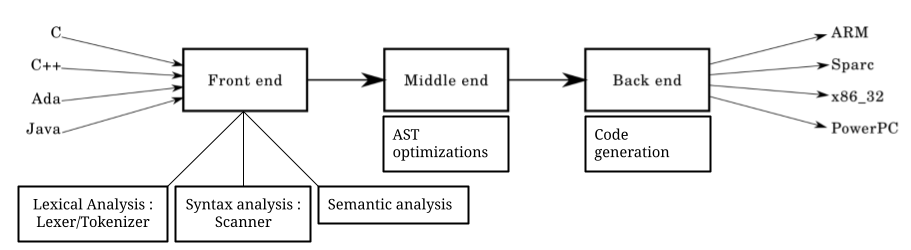
\includegraphics[width=\textwidth]{img/Compiler structure}
    \caption{Schematic representation of a classic compiler model\protect\footnotemark}
    \label{fig:compiler}
\end{figure}
\footnotetext{Modified image base on an illustration by Pronesto - File:Compiler design IPL.png, CC BY-SA 3.0, \url{https://commons.wikimedia.org/w/index.php?curid=49520771}}

\section{The initial situation}\label{sec:ch3-Parser}
As M. Mbonyincungu explains in his thesis~\cite{jpthesis}, creating a new syntax only makes sense if it can actually be used by programmers.
This requires the creation of some kind of program able to eventually transform \textit{NewOz} code into machine code.
Two possible approaches were identified : rewriting the existing \textit{Oz} compiler, \textit{ozc}, or creating a NewOz-to-Oz compiler.
M. Mbonyincungu decided to go with the second approach :
"One of the key elements of this project is that compatibility has to be maintained with the existing Mozart system, for the official release of Mozart2.
The idea of writing a new compiler has thus quickly been set aside, as it would drastically increase the time and complexity requirements of the project."~\cite{jpthesis}

Instead, that idea emerged of writing a "syntax parser" (\textit{sic}), that would serve as a compatibility layer between the \textit{NewOz} syntax, and the existing \textit{Oz} syntax supported by the current version of Mozart.
\textit{NewOz} code will be translated to the directly equivalent \textit{Oz} code, and then fed to the existing \textit{Oz} compiler, \texttt{ozc}.
Some readers might interject that this description lies closer to the definition of a compiler than a parser;
for this reason, we believe it is important to take the time and clarify the definition we give to each term in the context of this work.\newline

Wikipedia defines parsing as "the formal analysis by a computer of a sentence or other string of words into its constituents, resulting in a parse tree showing their syntactic relation to each other [\ldots]".~\cite{wikiParser}
A compiler, on the other hand, is described as "a computer program that translates computer code written in one programming language (the source language) into another language (the target language)."~\cite{wikiCompiler}
In my opinion, the program created by M. Mbonyincungu doesn't match any of those two definitions perfectly, as we will discuss below;
We think it lies somewhere in between those two definitions, as a decorator to the \texttt{ozc} compiler.
But to stay consistent with the terminology used in lest year's thesis and avoid confusion, we will refer to M. Mbonyincungu's program as "the Parser" in the rest of this document.\newline

M. Mbonyincungu's Parser makes use of \textit{Scala}'s Parsing Combinators library\footnote{See its documentation at \url{https://www.scala-lang.org/api/2.12.3/scala-parser-combinators/scala/util/parsing/combinator/Parsers.html}~\cite{ScalaParsers}}, which provides a syntax to match regular expressions and describe the relationship between them.
This library is used to describe pattern-matching rules which it then applied to the \textit{NewOz} code.
Finally, the \textit{Oz} code equivalent to each matched sentence was generated, with a great emphasis being put on maintaining the code's visual format.\footnote{See sections 3.2.3 and 3.3.1 of~\cite{jpthesis}}
This is important because the Parser was designed as a decorator to the Mozart compiler (which means that having code roughly at the same place will make debugging programs a lot easier), but also because it can prove useful in a teaching context in the future, when comparing the two syntax's side by side.\newline

This "parser approach" has been preferred over a rewrite/modification of the existing Mozart compiler for multiple reasons, which we will comment on in the next section :
\begin{enumerate}
    \item Because of its lower technical complexity, it would take less time to design;
    \item Working on an existing codebase could have revealed unforeseen problems and limitations;
    \item This approach would limit the amount of regression testing required;
    \item The use of a modern technology like \textit{Scala} would make the codebase easier to maintain and collaborate on;
    \item Future extensions and modifications would be easy, thanks to the inheritance concepts embedded in the library used.
\end{enumerate}
M. Mbonyincungu then describes the limitations and problems identified in his approach and implementation :
\begin{enumerate}[resume]
    \item The order in which some expressions alternations are declared in the pattern-matching code has a huge impact on the performance of the program.
    For example, if the code defines a statement of type A as \texttt{(p1 | p2)}, parsing \texttt{p2} in the code to compile is much more costly than parsing a statement \texttt{p1}.
    In practice, this results in much longer compilation time for the user, depending on the particular statements, expressions, or keywords they use.
    Based on my experience, this leads to a lot of confusion, as two programs of the same syntactic complexity can have drastically different compilation time.
    \item The Parser is stateless.
    This has a lot of implications, mainly when it comes to variable types;
    making it impossible, for example, to evaluate the validity of an arithmetic operation for two given arguments.
\end{enumerate}

\section{Limitations of the initial approach and proposed solution}\label{sec:ch3-problems}
To explain the thought process that led to the creation of \texttt{nozc}, we think it is important to firstly explain our interpretation and opinion on the points enumerated above.
Points 1 through 3 are very valid considerations when tackling a project of this size, especially in the context of a master thesis with limited time and a fixed deadline.
In that regard, the Parser is a great solution that accomplishes its objective : allowing programmers to test and run code written using the \textit{NewOz} syntax.\newline

However, since this work was placed in the direct continuation of M. Mbonyincungu's thesis, we had significantly more time to design a solution that is more ambitious technically and, we hope, easier to use.
In that context, points 4 and 5 were certainly taken into account : it is now clear that the \textit{NewOz} project's implementation will span multiple years, and it is essential to reduce the hand-over effort between maintainers to a minimum.
This implies, among other things, using popular technologies, maintaining a good documentation, writing modular and maintainable code, but also publishing it under an appropriate open-source license;
these considerations are further described in the next sections.
The problem identified in point 6 is in fact inherent to the library used;
as such, no amount of code optimization by the programmer could bring satisfactory results in that area.
This finding alone, in our opinion, revealed the need to have a new technical approach if we were to improve the \textit{NewOz} compiler.
Finally, the statelessness of the Parser also greatly limits the flexibility of the syntax in such a way that we could not consider it acceptable for real-world use.
This further reinforced our feeling that a new approach was necessary.\newline

Another big problem of the Parser that was mostly overlooked in last year's thesis, was the limited error reporting capabilities caused by the program's inherent structure.
As we said earlier, the Parser was designed to output \textit{Oz} code in a \texttt{.oz} file, and then execute the command-line \texttt{ozc} compiler with said file in input.
In practice, the Parser has limited semantic analysis capabilities, and this has two consequences.
First of all, it is enough to make us hesitant to call it as a proper compiler - as we touched upon earlier, even though it obviously does a lot more than a simple parser;
but more importantly, this limitation means that most errors will be caught during the second phase of the compilation, that is, during the execution of \texttt{ozc}.
This has the consequence that the user will receive messages describing errors present in the \textit{Oz} code, which might be quite different from the \textit{NewOz} code he wrote.
Moreover, we should remember that one of the goals of this approach was to make the intermediary "\textit{Oz} step" transparent to the user, and we can't expect future programmers, who will not have worked with Mozart/Oz, to know how to interpret \texttt{ozc} error messages.
Even though the Parser's output formatting does a great job at maintaining a visual equivalency between the \textit{NewOz} and \textit{Oz} versions of the code, some error messages will inevitably be undecipherable for the end user.
In my opinion, this limitation somehow defeats the purpose of making a new syntax and compiler in the first place, and is the main reason that pushed us to conceive a new solution involving a more complete compiler.

\section{A solution : \texttt{Nozc}}\label{sec:ch3-nozc}
The \textit{NewOz} Compiler~\cite{NozcGitHub}, which we decided to call \texttt{nozc} in reference to Mozart's \texttt{ozc} utility, is a complete compiler able to transform a \textit{NewOz} program written in a \texttt{.noz} file, into code executable using Mozart's \texttt{ozengine} command.
In that regard, it does not fit the most classic definition of a compiler, as we mentioned before, since it does not generate low-level machine code, but instead translates from one high-level language to another.
The current version of \texttt{nozc} runs on Windows, MacOS, and Linux, through a command-line interface.\newline

The overall approach used by this compiler is actually the same as the one imagined by M. Mbonyincungu for the Parser : the program will ingest a \texttt{.noz} file, write the equivalent \texttt{.oz} one, and then run \texttt{ozc} with that input.
However, we believe our approach is technically more accomplished, as it fully encompasses the 4 main phases of a classic compiler : lexer, parser, semantic analysis, and code generation, including a limited amount of optimization.
As such, it is able to produce informative, precise error messages that make debugging a \textit{NewOz} program a lot easier, without relying on the underlying \texttt{ozc} compiler.
In that regard, we believe it is a big improvement over last year's Parser, in the sense that it addresses our main criticism towards it.
The ultimate goal is to be able to handle in this compiler all warnings and errors, systematically generating \textit{Oz} code that will pass smoothly in the underlying \texttt{ozc} compiler every single time;
achieving this is essential if we want to mask the internal reliance on \texttt{ozc} to the end user.\newline

On top of its standard compilation functionality, \texttt{nozc} also provides other useful features, such as the ability to print the syntax tree of the program directly in the command-line, or to compile multiple files at a time.
Additionally, a couple of quality-of-life features have been embedded, such as a robust command-line interface that will make \texttt{nozc} easy to integrate in other tools by complying with general, good-practice CLI guidelines\footnote{More information on those practices can be found at \url{https://clig.dev/\#philosophy}~\cite{clig}}.
The user also has the ability to see the intermediary \textit{Oz} code generated during the compilation, or even to personalize the logging level of the output, by using the well-known Apache's Log4j logging levels\footnote{To be exact, \texttt{nozc} does not use Log4j, but adopted the same logging levels per convention. See \url{https://logging.apache.org/log4j/2.x/log4j-api/apidocs/org/apache/logging/log4j/Level.html} for a technical description of those levels and their meanings~\cite{log4j}}.\newline
\begin{figure}
    \centering
    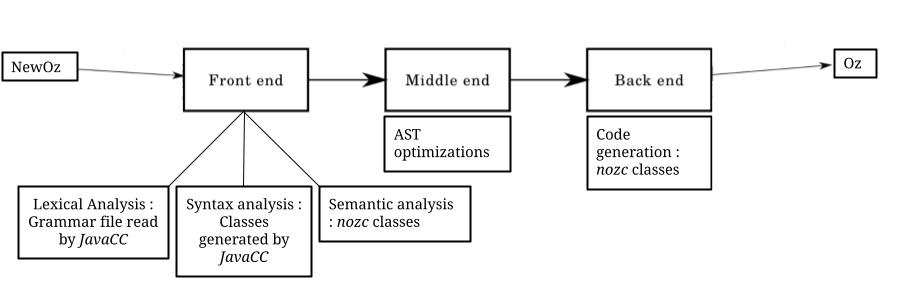
\includegraphics[width=\textwidth]{img/Compiler structure nozc}
    \caption{Schematic representation of the \texttt{nozc} compiler\protect\footnotemark}
    \label{fig:compilerNozc}
\end{figure}
\footnotetext{Modified image base on an illustration by Pronesto - File:Compiler design IPL.png, CC BY-SA 3.0, \url{https://commons.wikimedia.org/w/index.php?curid=49520771}}

The interested reader will find in Appendix~\ref{sec:appendix-compilation} a small example of the compilation process in \texttt{nozc}.

\section{Technologies used}\label{sec:ch3-technologies}
As said before, an important consideration when designing \texttt{nozc} was the maintainability of the project in the future.
Because this project will continue for multiple years and see different maintainers, it was important to select a technology that was either widespread and well known, or easy to apprehend, to future contributors to the project.
Another point of attention is the future support of the technologies chosen: again, later contributors should be able to find support and documentation easily.
For the programming language itself, our choice landed on \textit{Java}, more specifically the last version to date, JDK16.
Oracle's release cycle for Java has provided a major release every 6 months since September 2017, and it is a given at this point that Java will remain relevant for the years to come.
Other tools and libraries include :
\begin{itemize}
    \item Picocli, a framework for creating Java command line applications following POSIX conventions\footnote{The online documentation for Picocli is located at \url{https://picocli.info/}~\cite{picocli}}.
    A decisive factor in selecting this tool, apart from its very widespread use and great documentation, is the fact that it is designed to be shipped as a single \texttt{.java} file to include in the final application's source code.
    This means that upstream maintenance is not really a concern, as the source code is directly available to the programmer and can be easily be modified locally in the future, if necessary.
    \item JavaCC, a powerful parser generator creating a parser executable in a JRE\footnote{An overview of JavaCC's features can be found at \url{https://javacc.github.io/javacc/}~\cite{javacc}}.
    This tool is by far the most interesting improvement over last year's Parser.
    JavaCC provides a flexible and easy-to-use grammar to describe the grammar rules of the source language.
    This, along with its very complete documentation and wide community, means that a new maintainer should be able to quickly get a grip on this part of the compiler, which is the one most likely to be modified in the future, as we said before.
    JavaCC works by reading a grammar file, written by the user, describing the lexical and syntactic grammars of the language.
    It then automatically generates \textit{Java} classes describing a lexer and a parser, which can then be used to build the abstract syntax tree for valid programs, or report errors when needed.
    This solution saves a lot of time compared to writing a lexer and parser from scratch, with no identifiable drawbacks in our use case.
    \item Gradle\footnote{Gradle's homepage is located at \url{https://gradle.org/}~\cite{gradle}}, a building and packaging tool offering great documentation, regular updates and a powerful DSL, with built-in support in the most popular \textit{Java} IDEs.
    It is also designed to integrate automatically in any CD/CI pipeline.
    \item JUnit, the best unit testing framework for \textit{Java} programs.
    An additional library called System Rules\footnote{This collection of JUnit~\cite{JUnit} rules allows to test programs that make use of the \textit{System.exit()} instruction, allowing to test the correctness of the program's return codes directly from a JUnit test suite, without having to interrupt it. See \url{https://stefanbirkner.github.io/system-rules/index.html}~\cite{SystemRules}} was used for some specific test cases.
\end{itemize}
Overall, a great emphasis has been put on making \texttt{nozc} a future-proof and maintainable tool by : (a) using popular tools that, if they are not already mastered by future contributors, can be in a timely manner; (b) using tools that are actively maintained, reducing the risk associated with legacy code; (c) selecting trusted, open-source software, with licences that make them suited for use in our context; (d) limiting the amount of external tools, once again to reduce the risk of dependencies depreciation and other technical debt in the future.
The program itself is published on GitHub under the BSD license\footnote{This license is available for consultation at \url{https://github.com/MaVdbussche/nozc/blob/master/LICENSE}}.

\section{Evaluation of our approach}\label{sec:ch3-pros-cons}
We are convinced that the approach we selected with \texttt{nozc} makes it a great tool for the future contributors who would continue to work on \textit{NewOz}'s syntax in the coming years.
The modularity of the code makes it easy to add and remove language features without affecting others, while remaining flexible by making few assumptions about the language's grammar.
The code is also well documented, and we strongly believe that it can serve as a stepping stone towards the creation of a complete software ecosystem around \textit{NewOz}.
However, we have to mention limitations that we identified in our current implementation.\newline

The main one, in our opinion, is the inability of the compiler to print the generated \textit{Oz} code in a format that stays as close as possible to that of the source \textit{NewOz} code.
This is due to the fact that the lexer, in this particular implementation, ignores spaces and new line characters when reading the input.
This comes as a disadvantage compared to last year's Parser, but it also allows for a lot more flexibility in the way the programmer is allowed to format the source code.
This issue can raise some concerns, as we touched upon earlier : it implies that error messages generated by the underlying \texttt{ozc} compiler will most probably indicate an erroneous line and/or column number to the programmer.
However, this problem will progressively disappear over time with the maturation of \texttt{nozc}, as more and more of those errors will get caught in the first phase of the compilation.\newline

Another issue with of our approach lies in the fact that this compiler does not free itself from the dependency on the legacy \texttt{ozc}, which was one of our criticism towards M. Mbonyincungu's Parser implementation.
A more mature compiler should be able to generate machine code directly, or at the very least code that can be executed through Mozart's \texttt{ozengine} command, by itself, without relying on another piece of software.
As often seems to be the case in master theses however, time was a limiting factor;
supporting machine code generation for the various existing systems would take a lot of time and effort which we simply didn't have this year.
A solution to consider could be to rely on the JVM's multi-platform capabilities, by making \texttt{nozc} output JVM bytecode, effectively removing the need for  "manual" multi-platform support.
However, this approach would also come with its own drawbacks and difficulties, as some programming paradigms provided by \textit{Oz} and \textit{NewOz} will probably be difficult to support and implement on the JVM (in particular, one would lose Mozart's support for fine-grain threads, dataflow, and failed values)\footnote{Further reflections on this approach might benefit from reading the work of Sébastien Doeraene on Ozma~\cite{Ozma}}.
Another solution would be to fork the existing \texttt{ozc} compiler and modify its front-end to accept the new syntax, making, in a way, \texttt{nozc} the new front-end of \texttt{ozc}.\newline

But the main area of focus for future \texttt{nozc} improvements should probably be its integration in the existing Mozart environment through its Emacs interface.
The ability to compile regions of code directly from the Emacs editor is a major feature of \textit{Oz}, that has been left aside in this current implementation.
There are a lot of gains to be made here, especially from a teaching perspective.
This would probably be a massive undertaking though, and would require some knowledge of the Emacs system in general, and Mozart in particular.\newline

As you can see, even though we feel like this result is a significant improvement over last year's Parser, there still is a lot of work to be done before the publication of a first release version of \textit{nozc}.
We are confident however that the current \textit{beta} version is a significant first step in that direction.